\section{Introduction}\label{sec:intro}

\subsection{The problem}

Consider classical point particles of unit charge in $\R^3$, immersed in a uniform background of the opposite charge that makes the
system neutral. This is the \emph{jellium} or one-component plasma model. Wigner predicted that at low density the electrons of a
metal behave like such particles and form a crystal \cite{Wigner1934,Wigner1938}, and it has been believed since the first numerical
comparisons \cite{Fuchs1935} that the configuration of least energy at a given density is the body-centred cubic (BCC) lattice. A
proof would be an instance of the crystallization conjecture \cite{BlancLewin2015,Lewin2022}, which is open in three dimensions for
every long-range interaction. For Coulomb forces it is also delicate numerically: per particle, in units $e^2/a$ with $a$ the
Wigner--Seitz radius, the energies of the three classical candidates are \cite{BaikoPotekhinYakovlev2001}
\[
  \eB=-0.895929\ldots\ \text{(BCC)},\qquad \eF=-0.895873\ldots\ \text{(FCC)},\qquad -0.895838\ldots\ \text{(HCP)},
\]
so that the face-centred cubic (FCC) lattice and the hexagonal close-packed (HCP) structure lie above BCC by six and ten parts in
$10^5$ only.

Among \emph{lattices}, the energy per particle is the value at $s=\frac12$ of the analytic continuation of the Epstein zeta function
$\sum_{v\in\Lambda\setminus\{0\}}|v|^{-2s}$, up to normalization. Sarnak and Str\"ombergsson conjectured that at fixed covolume this
function is minimized by the BCC lattice for $0<s<\frac34$ and by the FCC lattice for $s>\frac34$, $s\ne\frac32$, the two lattices
having equal values at $s=\frac34$ \cite{SarnakStrombergsson2006}; at $s=\frac12$ both lattices are local minima, the FCC lattice by
\cite{Ennola1964Cambridge} and the BCC lattice by the duality $s\leftrightarrow\frac32-s$. In two dimensions the corresponding statement,
with the triangular lattice for all positive real $s$ and the finite part at the pole $s=1$, is classical
\cite{Rankin1953,Cassels1959,Ennola1964Glasgow,Diananda1964}; for a proof see \cite[Theorem~1 and the paragraph after it]{Montgomery1988}.
In three dimensions there has been decisive progress very recently: Luo and Wei proved the conjecture for the theta function and for
$s>\frac32$ \cite{LuoWei2026SS}, and Muratov and Novaga proved, with computer assistance, that the BCC lattice is the unique minimizer
of the Coulomb energy among all lattices \cite{MuratovNovaga2026}; see also \cite{LuoWei2026Yukawa}.

Lattices are a five-parameter family, and the real competitors of the BCC lattice are not all lattices: the HCP structure has two
particles per period cell. The natural next class consists of the periodic configurations with $N$ points per cell, $N=2,3,\dots$,
which exhaust all periodic configurations and, in a suitable sense, approximate all configurations. For the Coulomb energy, to our
knowledge, nothing has been proved in this direction; the comparison of BCC with HCP is numerical
\cite{Foldy1978,BaikoPotekhinYakovlev2001,BeterminSamajTravenec2023}. Muratov and Novaga single out the case $N=2$, with its five
shape and three position parameters, as an important intermediate step towards relaxing the assumption of periodicity
\cite[Section~7]{MuratovNovaga2026}. In this paper we settle this case, in a quantitative form.

\subsection{Results}

Let $e(X)$ denote the energy per particle of a periodic configuration $X\subset\R^3$, defined by Ewald summation
(Section~\ref{ssec:energy}); it scales like $e(tX)=t^{-1}e(X)$, and we fix the density to be $3/(4\pi)$. Let $\Ctwo$ be the set of
all configurations of this density that are lattices or unions $L\cup(L+\tau)$ of two translates of a lattice $L$. We say that $X$ is a
BCC (FCC) lattice if it is the image of the standard one under an isometry of $\R^3$, and we write $\eB$, $\eF$ for the two energies
and $\gap:=\eF-\eB=5.5640486\ldots\times10^{-5}$.

\begin{theorem}[Optimality]\label{thm:min}
For every $X\in\Ctwo$ we have $e(X)\ge\eB$, with equality if and only if $X$ is a BCC lattice.
\end{theorem}

The class $\Ctwo$ contains, besides all lattices, the HCP structures of all axial ratios, the diamond structure, and all structures
obtained from a lattice by displacing every second lattice plane. Theorem~\ref{thm:min} is a consequence of a sharper statement. In
Section~\ref{sec:defect} we define a \emph{defect} $D(X)\in[0,1]$. It is a local quantity: it compares the neighbours of a point of
$X$ within $1.3$ times the BCC cube side with the star of the fourteen nearest neighbours in a BCC lattice, optimally rotated; it
vanishes exactly on BCC lattices, it measures the squared deviation from the star as long as this is small, and it equals $1$ when
the neighbourhood is not a small deformation of the star, in particular for FCC and for HCP near the ideal axial ratio.

\begin{theorem}[Sharp stability]\label{thm:main}
For every $X\in\Ctwo$,
\begin{equation}\label{eq:main}
  e(X)-\eB\ \ge\ \gap\,D(X),
\end{equation}
with equality if and only if $X$ is a BCC lattice or an FCC lattice.
\end{theorem}

The constant $\gap$ is optimal, since $D=1$ on FCC lattices. Two consequences show what \eqref{eq:main} means without reference to the
details of $D$.

\begin{corollary}[FCC is optimal away from BCC]\label{cor:fcc}
If $X\in\Ctwo$ and $D(X)=1$, then $e(X)\ge\eF$, with equality if and only if $X$ is an FCC lattice.
\end{corollary}

For example, $D=1$ for the HCP structures with axial ratio near the ideal value $\sqrt{8/3}$, including the numerically minimizing
axial ratio, about $1.6356$ \cite{Sholl1967,Kozhberov2018}, for the diamond structure and for the simple cubic lattice
(Remark~\ref{rem:examples}). Thus every two-site configuration is either a small deformation of a BCC lattice, in the precise sense
$D<1$, or has energy at least $\eF$.

\begin{theorem}[Configurations below the FCC energy]\label{thm:basin}
Let $X\in\Ctwo$ with $e(X)<\eF$. Then $X$ is a deformed BCC lattice in the following sense. Let $\ltwo=(8\pi/3)^{1/3}$ and let
$\Bz=\Z^3\cup(\Z^3+(\frac12,\frac12,\frac12))$. There are a sublattice $L_0\subset\Bz$ of index two, a vector $w_0\in\Bz\setminus L_0$, a
matrix $A$ with $\det A=1$ and a vector $h\in\R^3$ such that, after a translation that moves a point of $X$ to the origin,
\[
  X=\ltwo\Bigl(AL_0\ \cup\ \bigl(AL_0+Aw_0+h\bigr)\Bigr),\qquad
  100\,\dist\bigl(A,\SO(3)\bigr)^2+200\,|h|^2\ \le\ D(X)\ \le\ \frac{e(X)-\eB}{\gap}\ <\ 1 ,
\]
where $\dist$ is the distance in the Frobenius norm.
\end{theorem}

Here $A$ is a homogeneous strain of the BCC lattice and $h$ a rigid displacement of one of its two sublattices with respect to the
other, in units of the cube side. Theorem~\ref{thm:basin} is a global version, valid on the whole sublevel set $\{e<\eF\}$, of the
statement that the BCC lattice is linearly stable under strains and under the zone-boundary phonons that preserve a sublattice of
index two. Its constants are explicit: $e-\eB\ge5.56\times10^{-3}\dist(A,\SO(3))^2+1.11\times10^{-2}\,|h|^2$. For comparison, the
second-order expansion of $e$ at the BCC lattice has, numerically, the coefficient $2.4\times10^{-2}$ for the softest strain and
$2.7\times10^{-2}$ for the softest sublattice displacement, so the global estimate is within a factor of five of the linearized one.

The restriction of Theorem~\ref{thm:main} to lattices (Theorem~\ref{thm:bravais}) is an ingredient of the proof and may be of
independent interest: it contains the theorem of Muratov and Novaga, with an independent proof, and it adds the stability estimate
and the characterization of the FCC lattice as the only other equality case. For lattices the theorem is, moreover, verified in a
proof assistant, with a separate certificate; see Sections~\ref{ssec:verification} and~\ref{ssec:lean}.

\subsection{Remarks}

\emph{On the defect.} Inequalities of the form ``energy excess $\ge$ constant $\times$ number of defects'' are the mechanism of the
known crystallization proofs for short-range interactions \cite{Theil2006,FlatleyTheil2015}. A functional like $D$ is needed to state
such an inequality for an energy that has no nearest-neighbour structure, and the particular $D$ of Section~\ref{sec:defect} is
designed to be meaningful for arbitrary configurations, where it is defined at every point. Its definition involves a few numerical
parameters, and the sharp form of \eqref{eq:main} depends on them; Theorem~\ref{thm:min}, Corollary~\ref{cor:fcc} and
Theorem~\ref{thm:basin} are the robust consequences. For configurations in $\Ctwo$ with $D<1$ we compute $D$ exactly
(Theorem~\ref{thm:registration}): it is $100\dist(A,\SO(3))^2+200|h|^2$ plus a penalty for neighbours that do not belong to the
deformed star, and the penalty vanishes for $D\le0.52$.

\emph{On the equality cases.} The deficit $e-\eB-\gap D$ vanishes exactly on the BCC and the FCC lattice, up to isometry, and is
nowhere negative. Along the Bain path, the family of body-centred tetragonal lattices that joins BCC to FCC, the energy excess rises
to $2.6\,\gap$ before it returns to $\gap$ at the FCC lattice (Figure~\ref{fig:bain}); the BCC and FCC lattices are separated by a
barrier, and what the theorem expresses is that the valley floor at the FCC lattice, at height exactly $\gap$, lies outside the BCC
basin $\{D<1\}$, and that nothing outside this basin lies lower.

\emph{Other work beyond lattices.} For other energies there are results on periodic configurations with several points per cell:
local optimality of certain lattices among all periodic sets \cite{CoulangeonSchurmann2012,CoulangeonSchurmann2021}, the comparison of
FCC and HCP for completely monotone summable potentials within stackings of triangular layers \cite{BeterminPetrache2017}, numerical
searches \cite{CohnKumarSchurmann2009}, and, very recently, the optimality of BCC for the quantization energy among two-site
configurations with a rectangular period cell, together with a sharp stability constant for its second variation
\cite{LuoXie2026}, and the local minimality of BCC for a quantization functional under small periodic perturbations
\cite{AydinIacobelli2026}. None of these covers the Coulomb energy. To our knowledge, Theorems~\ref{thm:min}--\ref{thm:basin} are the first
optimality results beyond lattices, and the first global stability inequality, for the three-dimensional Coulomb energy.

\begin{figure}[h]
\centering
% Generated from floating-point data (illustration only; not used in any proof).
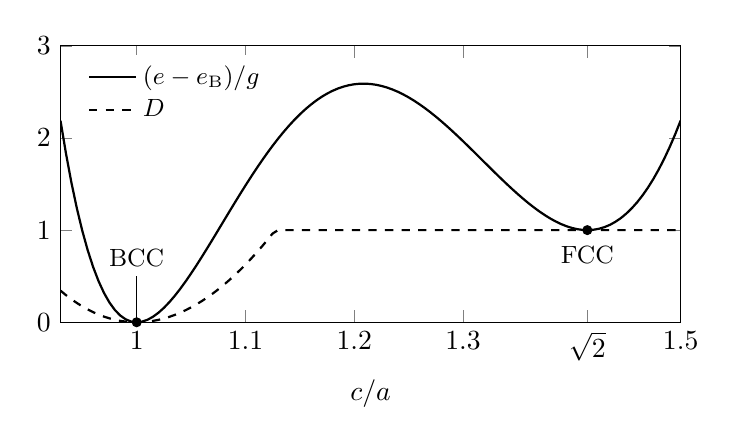
\begin{tikzpicture}
\begin{axis}[width=0.78\textwidth,height=0.42\textwidth,xmin=0.93,xmax=1.5,ymin=0,ymax=3,
  xlabel={$c/a$},ylabel={},xtick={1,1.1,1.2,1.3,1.4142,1.5},xticklabels={$1$,$1.1$,$1.2$,$1.3$,$\sqrt2$,$1.5$},
  ytick={0,1,2,3},legend pos=north west,legend cell align=left,legend style={draw=none,font=\small}]
\addplot[thick,black] coordinates {
(0.930,2.1877) (0.935,1.8328) (0.940,1.5171) (0.945,1.2382) (0.950,0.9938) (0.955,0.7816) (0.960,0.5995) (0.965,0.4455) (0.970,0.3176) (0.975,0.2140) (0.980,0.1328) (0.985,0.0725) (0.990,0.0312) (0.995,0.0076) (1.000,0.0000) (1.005,0.0071) (1.010,0.0275) (1.015,0.0600) (1.020,0.1033) (1.025,0.1563) (1.030,0.2178) (1.035,0.2868) (1.040,0.3623) (1.045,0.4435) (1.050,0.5293) (1.055,0.6189) (1.060,0.7117) (1.065,0.8067) (1.070,0.9034) (1.075,1.0011) (1.080,1.0992) (1.085,1.1970) (1.090,1.2941) (1.095,1.3900) (1.100,1.4842) (1.105,1.5763) (1.110,1.6659) (1.115,1.7526) (1.120,1.8361) (1.125,1.9162) (1.130,1.9926) (1.135,2.0649) (1.140,2.1331) (1.145,2.1970) (1.150,2.2563) (1.155,2.3109) (1.160,2.3608) (1.165,2.4059) (1.170,2.4461) (1.175,2.4813) (1.180,2.5115) (1.185,2.5367) (1.190,2.5570) (1.195,2.5723) (1.200,2.5828) (1.205,2.5884) (1.210,2.5893) (1.215,2.5856) (1.220,2.5773) (1.225,2.5646) (1.230,2.5476) (1.235,2.5265) (1.240,2.5015) (1.245,2.4726) (1.250,2.4402) (1.255,2.4043) (1.260,2.3653) (1.265,2.3232) (1.270,2.2784) (1.275,2.2310) (1.280,2.1813) (1.285,2.1296) (1.290,2.0761) (1.295,2.0210) (1.300,1.9647) (1.305,1.9073) (1.310,1.8492) (1.315,1.7907) (1.320,1.7321) (1.325,1.6736) (1.330,1.6155) (1.335,1.5582) (1.340,1.5019) (1.345,1.4470) (1.350,1.3938) (1.355,1.3425) (1.360,1.2935) (1.365,1.2472) (1.370,1.2038) (1.375,1.1637) (1.380,1.1272) (1.385,1.0946) (1.390,1.0663) (1.395,1.0426) (1.400,1.0237) (1.405,1.0102) (1.410,1.0022) (1.415,1.0001) (1.420,1.0042) (1.425,1.0150) (1.430,1.0326) (1.435,1.0575) (1.440,1.0900) (1.445,1.1303) (1.450,1.1789) (1.455,1.2361) (1.460,1.3022) (1.465,1.3775) (1.470,1.4623) (1.475,1.5570) (1.480,1.6620) (1.485,1.7774) (1.490,1.9037) (1.495,2.0411) (1.500,2.1901)
};
\addlegendentry{$(e-e_{\mathrm B})/g$}
\addplot[thick,black,dashed] coordinates {
(0.930,0.3430) (0.935,0.2947) (0.940,0.2502) (0.945,0.2094) (0.950,0.1725) (0.955,0.1392) (0.960,0.1096) (0.965,0.0836) (0.970,0.0612) (0.975,0.0424) (0.980,0.0270) (0.985,0.0152) (0.990,0.0067) (0.995,0.0017) (1.000,0.0000) (1.005,0.0017) (1.010,0.0066) (1.015,0.0149) (1.020,0.0263) (1.025,0.0410) (1.030,0.0588) (1.035,0.0798) (1.040,0.1039) (1.045,0.1311) (1.050,0.1613) (1.055,0.1946) (1.060,0.2309) (1.065,0.2702) (1.070,0.3123) (1.075,0.3574) (1.080,0.4055) (1.085,0.4563) (1.090,0.5101) (1.095,0.5666) (1.100,0.6259) (1.105,0.6881) (1.110,0.7529) (1.115,0.8205) (1.120,0.8908) (1.125,0.9637) (1.130,1.0000) (1.135,1.0000) (1.140,1.0000) (1.145,1.0000) (1.150,1.0000) (1.155,1.0000) (1.160,1.0000) (1.165,1.0000) (1.170,1.0000) (1.175,1.0000) (1.180,1.0000) (1.185,1.0000) (1.190,1.0000) (1.195,1.0000) (1.200,1.0000) (1.205,1.0000) (1.210,1.0000) (1.215,1.0000) (1.220,1.0000) (1.225,1.0000) (1.230,1.0000) (1.235,1.0000) (1.240,1.0000) (1.245,1.0000) (1.250,1.0000) (1.255,1.0000) (1.260,1.0000) (1.265,1.0000) (1.270,1.0000) (1.275,1.0000) (1.280,1.0000) (1.285,1.0000) (1.290,1.0000) (1.295,1.0000) (1.300,1.0000) (1.305,1.0000) (1.310,1.0000) (1.315,1.0000) (1.320,1.0000) (1.325,1.0000) (1.330,1.0000) (1.335,1.0000) (1.340,1.0000) (1.345,1.0000) (1.350,1.0000) (1.355,1.0000) (1.360,1.0000) (1.365,1.0000) (1.370,1.0000) (1.375,1.0000) (1.380,1.0000) (1.385,1.0000) (1.390,1.0000) (1.395,1.0000) (1.400,1.0000) (1.405,1.0000) (1.410,1.0000) (1.415,1.0000) (1.420,1.0000) (1.425,1.0000) (1.430,1.0000) (1.435,1.0000) (1.440,1.0000) (1.445,1.0000) (1.450,1.0000) (1.455,1.0000) (1.460,1.0000) (1.465,1.0000) (1.470,1.0000) (1.475,1.0000) (1.480,1.0000) (1.485,1.0000) (1.490,1.0000) (1.495,1.0000) (1.500,1.0000)
};
\addlegendentry{$D$}
\addplot[only marks,mark=*,mark size=1.6pt,black] coordinates {(1,0) (1.41421,1)};
\node[anchor=south,font=\small] at (axis cs:1,0.5) {BCC};
\draw[thin] (axis cs:1,0.5) -- (axis cs:1,0.05);
\node[anchor=north,font=\small] at (axis cs:1.41421,0.93) {FCC};
\end{axis}
\end{tikzpicture}

\caption{Body-centred tetragonal lattices of axial ratio $c/a$ (in units in which BCC is $c/a=1$ and FCC is $c/a=\sqrt2$): the
energy excess $(e-\eB)/\gap$ (solid) and the defect $D$ (dashed). The inequality \eqref{eq:main} says that the solid curve lies above
the dashed one; they touch at the two cubic lattices. The figure is a numerical illustration, computed in floating-point
arithmetic, and is not used in any proof.}\label{fig:bain}
\end{figure}

\subsection{Strategy of the proof}

The proof has an analytic part, which reduces the theorem to finitely many inequalities, and a computational part, which verifies
them.

\emph{A positive series.} Ewald's formula with a suitable splitting parameter expresses $e(X)$ through a series all of whose terms
are nonnegative (Proposition~\ref{prop:series}). Hence every partial sum is a rigorous lower bound for the energy, and convexity
properties of the terms can be exploited freely. This representation is due to Riemann for the zeta function and was used in
\cite{SarnakStrombergsson2006,MuratovNovaga2026} for lattices.

\emph{Compactness.} If the period lattice has a short vector, or if two points are close, a single term of the series already exceeds
the FCC energy. Together with lattice reduction this confines every possible violation of \eqref{eq:main} to a box
$\Kbox\subset\R^8$ with rational vertices (Proposition~\ref{prop:compact}).

\emph{The defect.} For $D<1$ the minimization that defines $D$ is solved by a unique ``registration'' of the configuration on a
BCC lattice (Theorem~\ref{thm:registration}). Since every trial gives an upper bound for $D$, one registration chosen for a box gives
upper bounds for $D$ on the whole box, and these are tight near the BCC lattices.

\emph{The equality cases.} Each of the two cubic lattices has seven descriptions as a two-site configuration, one for every
sublattice of index two. At each of the fourteen points the deficit vanishes to second order. We expand it to fourth order with
certified bounds for the Hessian and for the third and fourth derivatives, and obtain \eqref{eq:main} in an explicit neighbourhood
(Theorem~\ref{thm:local}). The proof of the main theorems does not need this local result: the comparison with lattices described
next also covers these neighbourhoods.

\emph{Lattices as anchors.} The lattices form the five-dimensional set $\{2\tau\in L\}$ inside $\Ctwo$. Near this set, bounds that
treat the energy and the defect separately cannot resolve the deficit wherever the deficit of the nearby lattices is small, in
particular around the BCC and FCC lattices. We first prove \eqref{eq:main} for lattices
(Theorem~\ref{thm:bravais}), and then extend it to a neighbourhood of the set of lattices by comparing a configuration
$L\cup(L+\tau)$ with the lattice $L\cup(L+\tau_0)$, $\tau_0\in\frac12L$, nearest to it: the energy grows at least quadratically in
$\tau-\tau_0$, with a rate that we bound from below on boxes, while the defect grows at most quadratically, with a rate controlled
by the registration theorem (Section~\ref{ssec:anchor}).

\emph{The cover.} The rest of $\Kbox$ is covered by boxes on which the inequality holds with a positive margin, either because the
energy exceeds $\eF$ or because a lower bound for the energy exceeds an upper bound for $\eB+\gap D$. The lower bounds combine the
logarithmic convexity of the terms of the series, separate convexity of the squared lengths in the coordinates of $\Kbox$, which
reduces a bound on a box to its $256$ vertices, and a planar summation formula for configurations made of well separated layers
(Section~\ref{sec:cover}). The cover was produced adaptively, in ten stages; Table~\ref{tab:stages} lists the certificate that was
verified, by stage.

\subsection{Computer assistance and verification}\label{ssec:verification}

The proofs of Theorems~\ref{thm:bravais}, \ref{thm:local} and~\ref{thm:cover} depend on computations: enclosures of the constants
$\eB$ and $\eF$, and inequalities on more than seventeen million boxes. All of them are carried out in ball arithmetic with rigorous
error bounds, using the Arb library \cite{Johansson2017Arb,flint}, on data with exact rational endpoints; floating-point numbers are
used only to guide the search. The result is a certificate, a collection of files that record, for each box, which of the
sufficient conditions of Section~\ref{sec:cover} holds and with which parameters, together with a program, separate from those that
produced the cover (it neither imports nor calls them), that verifies the recorded inequalities and the completeness of the cover
(Section~\ref{ssec:certs}). In this respect the proof is of the same nature as other computer-assisted proofs in discrete geometry
and analysis \cite{Hales2005,MuratovNovaga2026}. Section~\ref{sec:computation} describes the certificate, the precision used, the
checks that were performed, and what remains to be trusted.

Part of the argument has in addition been formalized in the Lean~4 proof assistant \cite{deMouraUllrich2021} with the Mathlib library
\cite{mathlib2020}: the lattice case, Theorem~\ref{thm:bravais}, is proved there completely, with a certificate of its own that is
evaluated by the Lean kernel, and so are parts of the two-site argument, among them the reduction to the box $\Kbox$ and the bounds
for the defect. The cover of $\Kbox$ is checked by the program just described and not in the proof assistant, so that for general
two-site configurations Theorem~\ref{thm:main} is a computer-assisted theorem in the usual sense; the precise scope of the
formalization is stated in Section~\ref{ssec:lean}.

\subsection{Organization}

Sections~\ref{sec:setting}--\ref{sec:reduction} define the energy and the defect and reduce the theorem to the box $\Kbox$;
Sections~\ref{sec:bravais} and~\ref{sec:local} treat lattices and the neighbourhoods of the equality cases; Section~\ref{sec:cover}
describes the cover and Section~\ref{sec:proof} completes the proofs. Section~\ref{sec:computation} reports on the computations and
their verification, and Section~\ref{sec:outlook} on open problems. Appendix~\ref{app:ewald} proves Ewald's formula, and
Appendices~\ref{app:tails} and~\ref{app:details} give the technical bounds in full.
